\documentclass[12pt,a4paper]{article}
\usepackage[utf8]{inputenc}
\usepackage[UKenglish]{babel}
\usepackage[T1]{fontenc}
\usepackage{microtype}
\usepackage{graphicx}
\usepackage{amsmath}
\usepackage{lmodern}
\usepackage{indentfirst}
\usepackage{setspace}
\usepackage{tabularx}
\usepackage{caption}
\usepackage{subcaption}
\usepackage{enumitem}

%\usepackage{times}
\usepackage[hyphenbreaks]{breakurl}
\usepackage[hyphens]{url}
\usepackage[left=3cm,right=2cm,top=2cm,bottom=2cm]{geometry}
\usepackage[style=numeric,backend=bibtex]{biblatex}
\usepackage[nottoc,numbib]{tocbibind}
%\addbibresource{cit.bib}
\renewcommand\_{\textunderscore\allowbreak}
\usepackage{float}
\author{Abraham Lenson}
\title{Online Text Editor}
\begin{document}
%\maketitle

\setlength{\parskip}{.5\baselineskip}

\raggedleft
\Huge Online Text Editor\\~\\
\Large Abraham Lenson\\
%\large 341946\\
\large Rustenis Tolpežnikas\\
%\large 
\raggedright

\tableofcontents\newpage

\spacing{1.15}

\section{Introduction}
This report documents the implementation of our online distributed text editor implementation.  Starting from concept design, revisions and changes, and our general testing process.  This report will heavily reference our previous concept design document as it is the basis of our project.


\section{General Assumption}
The goal of this project is to develop a Decentralized Online Text Editor. Here are the requirements given specifically to this project:

\begin{itemize}
\item Each user of the editor should be able to see the current state of the edited document, can edit and erase the text.\\
\item There should be cursors visible to all users, symbolizing where other editors are currently positioned in the document (in other terms, which portion are they currently editing).\\
\end{itemize}

Furthermore, there were general requirements given to all the projects of this course:

\begin{itemize}
\item The developed system should be multi-node. Two or more computers should constitute the nodes; additional nodes can run in VMs or similar containers.\\
\item The system should have a multi-part design, as we are a 2-person team, this would mean 2 parts.\\
\item Each part should work on a different OS and be written in a different language.\\
\item The system should have some fault tolerance, such as handling network disconnection and node failure, as well as not reset after a malfunction and restore the distributed state at least partially.\\
\end{itemize}


Given these initial requirements, in team we have decided that the 2 parts will be 2 similar but different implementations of the individual nodes. We prepared a backend node and a frontend node. The backend communicates with each other while the frontend handles the UI and could accept multiple clients.

For the system to work on different OS systems, we would be developing the 2 different node implementations in programming languages known to be OS-agnostic (such as Python, JavaScript, etc.).

Given these initial requirements and the defined general assumptions, we can categorize the requirements and refine them:
\begin{tabularx}{\textwidth}{|l|l|X|}
\hline
RE1 & Real-Time Sync & All nodes must synchronize text edits in real-time. \\
\hline
RE2 & Multi-Node Support & System must support at minimum 3 connected nodes, without a hard upper limit (but soft limit could be stated as 10). \\
\hline
RE3 & Cursor Visibility & Remote cursors must be visible to all users with positional updates. \\
\hline
RE4 & Editor UI & Provide a functional editor interface, which can be used to edit (insert, delete, select) the text. \\
\hline
RE5 & Dynamic Election & If a distinguished node exists, elect a new leader upon failure. \\
\hline
NRE1 & Cross-Platform & The implementation of the node should not be limited to a single programming language, and it should be possible to run the system on different Operating Systems. \\
\hline
NRE2 & Fault Tolerance & System must recover from node/network failures without full reset (partial state restore). \\
\hline
NRE3 & Debug Mode & The system should provide access to its inner state for the sake of debugging. \\
\hline
\end{tabularx}
\newpage
\section{Technology Stack}
In order to implement the system, we need to make sure that the data are synchronised correctly across different clients. To do that, we need a framework to deal with state changes, desynchronization, merge conflicts, and other issues that may arise from a decentralised system. To deal with that we are going to use CRDTs (Conflict-Free Replicated Data Types), a data structure that allow distributed systems to sync seamlessly without coordination and ensuring eventual consistency. They handle concurrent edits by making all operations commutative, associative, and idempotent.

Due to the cross-language and cross-platform approach required, we scrapped our original idea of using YATA based approaches.  Instead, we keep things mostly simple with a Last-Write-Wins based approach through websocket.  This generally works pretty well over a local network, and generally doesn't encounter issue such as tombstoning or bloating from previously deleted elements.

\newpage
\section{System Architecture}
\textbf{Abstract top-down view of the system:}

\begin{figure}[H]
\caption{Abstract}
\centering
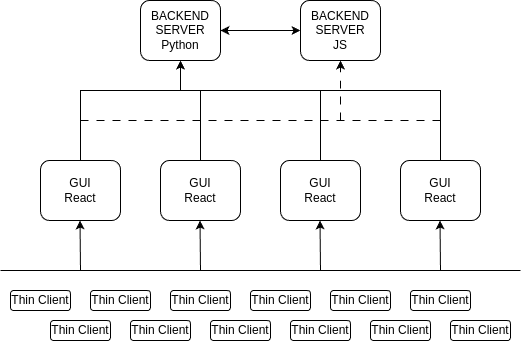
\includegraphics[width=0.7\textwidth]{topdown.drawio}
\end{figure}

\textbf{Key concepts explained:}
\begin{tabularx}{\textwidth}{|l|X|}
    \hline
    \textbf{Concept} & \textbf{Description} \\
    \hline
    GUI Server & 
    \begin{itemize}[nosep, left=0pt]
        \item Allows the client to see the up-to-date version of the document.
        \item Enables the textual editing of the said document.
        \item Shows the concurrent user sessions as cursors.
        \item Handles Document Processing
    \end{itemize} \\
    \hline
    Backend Server & 
    \begin{itemize}[nosep, left=0pt]
        \item Bridges to the GUI Server through WebSocket layer
        \item Handles synchronisation between clients
        \item Switches Role between backup and main server depending on server status
    \end{itemize} \\
    \hline
    Websocket & 
    \begin{itemize}[nosep, left=0pt]
        \item Standardized message format
        \item Routes messages between language backends
        \item Handles connection state management
    \end{itemize} \\
    \hline
    Thin Clients & 
    \begin{itemize}[nosep, left=0pt]
        \item Shows UI through a browser
        \item Handles User Input
    \end{itemize} \\
    \hline
\end{tabularx}


\section{Behavioral Diagrams}
\subsection{Sequence Diagram}
\begin{figure}[H]
\caption{Sequence Diagram}
\centering
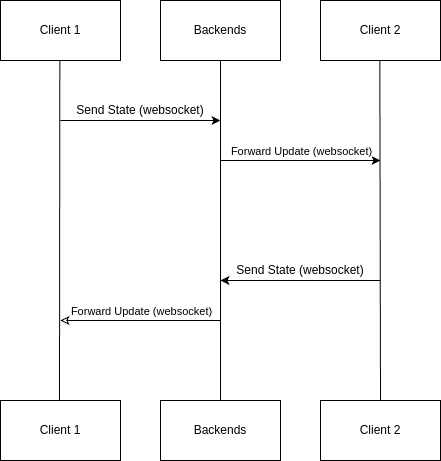
\includegraphics[width=0.6\textwidth]{seq.drawio}
\end{figure}

\newpage
\section{Testing}

To evaluate the system’s reliability, real-time synchronization, and multi-node support, we set up a controlled networked environment. The testbed consisted of multiple laptops connected within a single local area network (LAN). The setup included two backend server nodes and several frontend client nodes, each running on different operating systems to comply with the cross-platform requirement.

Each server node handled backend logic, synchronization, and message routing, while the client nodes provided the editor interface and user interaction. We connected additional laptops to the client nodes to simulate concurrent usage by multiple users.

During the test, users simultaneously edited shared documents. Edits included insertions, deletions, and cursor movements. The system successfully synchronized changes in real-time across all connected nodes. Cursor positions were updated accurately and promptly, reflecting each user’s activity.

We also introduced basic fault scenarios, such as temporarily disconnecting a node. The system managed to recover without a full reset and restored a partially consistent state, validating our fault-tolerance assumptions.

Overall, the system operated as expected under realistic network conditions, meeting the key functional and non-functional requirements outlined in our design.
\newpage
\nocite{*}%cite all in bibliography
\printbibliography

\addcontentsline{toc}{section}{References}

\end{document}
